% Mid-term draft of the research paper (ACM acmart, same style as the course template).
% Build locally:  tectonic main.tex     (or upload this folder to Overleaf)
% Red [square-bracket] text marks what the team must still fill in.
% `nonacm` removes the ACM copyright/reference blocks, which a course paper does not need.
\documentclass[acmtog,nonacm]{acmart}

\usepackage{array}
\usepackage{tikz}
\usetikzlibrary{decorations.pathreplacing}

% Colour name in capitals: acmart upper-cases author names, which would turn `red' into `RED'.
\definecolor{PH}{rgb}{0.80,0.05,0.05}
\newcommand{\placeholder}[1]{{\color{PH}[#1]}}
% Ragged-right table column of a given width.
\newcolumntype{L}[1]{>{\raggedright\arraybackslash}p{#1}}
% Let TeX stretch spaces a little more rather than overflow the narrow columns.
\setlength{\emergencystretch}{2em}

\begin{document}

\title{Staying in Touch, Simply}
\subtitle{Co-Designing a Way for an Older Adult to Use His Smartphone (mid-term draft)}

\author{Henrique Rodrigues}
\affiliation{%
  \institution{Instituto Superior T\'ecnico, Universidade de Lisboa}
  \city{Lisbon}
  \country{Portugal}}
\author{Jo\~ao Rocha}
\affiliation{%
  \institution{Instituto Superior T\'ecnico, Universidade de Lisboa}
  \city{Lisbon}
  \country{Portugal}}

\renewcommand{\shortauthors}{Rodrigues and Rocha}

\begin{abstract}
Many older adults own a smartphone they cannot use. We are co-designing, with Manuel, an 80-year-old man in Lisbon, a way for him to use the smartphone his daughter bought him so he could follow the family's WhatsApp group. He does not want a simpler phone: he wants the smartphone's family features, photos, messages and news, without having to learn how to work it. This mid-term draft covers related work, secondary research on older adults in Portugal, our method, and the first two of three co-design sessions, in which Manuel framed the problem and chose a concept: a plain cover that shows one thing at a time, with a green button to talk and a red one to end.
\end{abstract}

\ccsdesc[500]{Human-centered computing~Accessibility technologies}
\ccsdesc[300]{Human-centered computing~Participatory design}
\ccsdesc[300]{Human-centered computing~Mobile devices}

\keywords{co-design, older adults, inclusive design, smartphones, voice interaction}

\maketitle

\section{Introduction}
Smartphones are now where many families share news and photos, but many older adults find them hard to learn and easy to get wrong~\cite{kurniawan2008older, leung2012older}. In Portugal, which has the second-oldest population in the EU, only one in five people aged 65--74 has at least basic digital skills~\cite{eurostat2025population, eurostat2025digitalskills}.

Rather than designing for older adults, we design with one of them~\cite{sanders2008cocreation}. Over three sessions following the Double Diamond~\cite{designcouncil2004double}, Manuel defines the problem with us, creates and chooses ideas, and will test our prototype at home. This draft covers the first two sessions.

\section{Related Work}\label{sec:related}

\subsection{Older adults and smartphones}
Older adults are not simply afraid of technology: they weigh its benefits against its hassle~\cite{mitzner2010older}, and anxiety and confidence, more than age itself, predict whether they adopt it~\cite{czaja2006factors}. Touchscreens remain a barrier. Older adults' typing errors on touchscreens rise with hand tremor~\cite{nicolau2012elderly}, and flat designs make it harder for them to tell what can be pressed~\cite{urbano2022skeuomorphism}. Senior launchers make the screen simpler, but fewer features alone do not make a phone usable~\cite{petrovcic2018smart}.

\subsection{Voice interaction}
Voice assistants can reach older adults who avoid screens, but they are abandoned when people find few valuable uses~\cite{trajkova2020alexa}, reminders go unused when people doubt them~\cite{pradhan2020use}, and recognition errors become the main frustration over time~\cite{kim2021exploring}. A voice interface should do a few things the person values and recover gracefully from mistakes.

\subsection{Co-design and stigma}
Co-design treats the people who will use a design as co-creators~\cite{sanders2008cocreation}, and participatory and generative methods help older people take part from the start~\cite{lindsay2012engaging, andersen2019magic}. Designs must also avoid stigma: devices that mark their users as old or disabled are often rejected~\cite{shinohara2011shadow, neven2010obviously}.

\section{Methodology}\label{sec:method}

\begin{figure}[t]
  \centering
  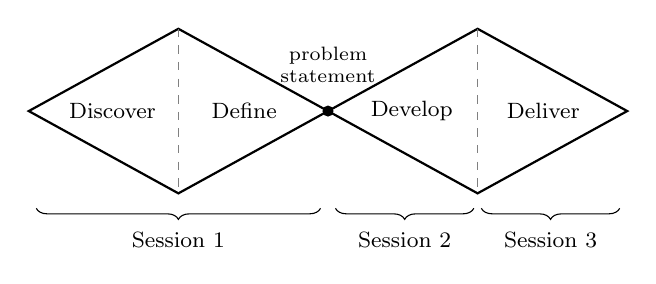
\begin{tikzpicture}[x=0.95cm, y=0.95cm, font=\footnotesize]
    \draw[thick] (0,0) -- (2,1.1) -- (4,0) -- (2,-1.1) -- cycle;
    \draw[thick] (4,0) -- (6,1.1) -- (8,0) -- (6,-1.1) -- cycle;
    \draw[dashed, gray] (2,1.1) -- (2,-1.1);
    \draw[dashed, gray] (6,1.1) -- (6,-1.1);
    \node at (1.12,0) {Discover};
    \node at (2.88,0) {Define};
    \node at (5.12,0) {Develop};
    \node at (6.88,0) {Deliver};
    \fill (4,0) circle (2pt);
    \node[align=center, font=\scriptsize] at (4,0.62) {problem\\statement};
    \draw[decorate, decoration={brace, mirror, amplitude=4pt}] (0.1,-1.3) -- (3.9,-1.3)
      node[midway, below=5pt] {Session 1};
    \draw[decorate, decoration={brace, mirror, amplitude=4pt}] (4.1,-1.3) -- (5.95,-1.3)
      node[midway, below=5pt] {Session 2};
    \draw[decorate, decoration={brace, mirror, amplitude=4pt}] (6.05,-1.3) -- (7.9,-1.3)
      node[midway, below=5pt] {Session 3};
  \end{tikzpicture}
  \caption{Our three co-design sessions mapped onto the Double Diamond.}
  \Description{Two diamonds side by side, divided into four stages labelled Discover, Define, Develop and Deliver. The point where the diamonds meet is labelled problem statement. Braces underneath mark Session 1 under the whole first diamond, Session 2 under Develop and Session 3 under Deliver.}
  \label{fig:diamond}
\end{figure}

\subsection{Co-designer}
Manuel is 80, a widower and a retired electrician, and lives alone in Lisbon; his daughter introduced him to us. He calls his family every day on a button phone. In July, his daughter bought him a smartphone so he could join the family's WhatsApp group, where photos of his newborn great-grandson are shared. He does not know how to work it, so it stays in a drawer.

\subsection{Sessions}
We follow the Double Diamond (Figure~\ref{fig:diamond}). Each session takes about 70 minutes in Manuel's kitchen. In session~1 we used directed storytelling, a tour of both his phones and a communication map, and wrote the problem statement with him. In session~2 he sorted 16 action cards, compared three empty 3D-printed mock-ups, acted out the phone's behaviour while a teammate played its voice, and narrated a storyboard. Session~3 will test our prototype.

We adapted the sessions to him: he hosted a card game before any question, we read the consent form aloud in plain Portuguese, and only one of us asked at a time. With his consent, we took notes, recorded audio and photographed his hands and materials, never his face, and we analyse them with thematic analysis~\cite{braun2006using}. Participation follows a project declaration signed by Manuel and the team; recordings will be deleted by \placeholder{date}.

\section{Secondary Research}\label{sec:secondary}
Older adults in Portugal are less connected than their European peers (Table~\ref{tab:stats}), but those who are online message and call more than the EU average, so staying in touch is a central use.

\begin{table}[t]
  \caption{Older adults in Portugal and the EU-27, Eurostat 2025~\cite{eurostat2025population, eurostat2025internet, eurostat2025digitalskills, eurostat2025activities, eurostat2025livingalone}.}
  \label{tab:stats}
  \small
  \begin{tabular}{@{}L{0.62\columnwidth}rr@{}}
    \toprule
    Indicator & Portugal & EU-27 \\
    \midrule
    Population aged 65 or over & 24.3\% & 22.0\% \\
    Never used the internet, ages 65--74 & 36.1\% & 16.4\% \\
    At least basic digital skills, ages 65--74 & 20.7\% & 33.0\% \\
    Instant messaging, internet users aged 65--74 & 79.8\% & 74.5\% \\
    People aged 65 or over living alone & 25.7\% & 32.2\% \\
    \bottomrule
  \end{tabular}
\end{table}

Existing products do not fit Manuel. Minimal phones such as the Light Phone drop apps like WhatsApp~\cite{light2026phoneiii}. Simplified modes such as Samsung's Easy mode only change how the phone looks, and Apple's Assistive Access leaves apps like WhatsApp in their usual design~\cite{samsung2026easymode, apple2026aaapps}. Mainstream voice assistants do not support European Portuguese~\cite{pplware2021alexa, google2026nestlanguages}.

\section{Early Findings}\label{sec:findings}

\subsection{Session 1}
\begin{itemize}
  \item \emph{He cannot work the smartphone.} His taps were too short, a pinch shrank the text and the keyboard opened by accident: ``I broke the letters. Put them back.''
  \item \emph{But he wants what is inside it.} He will not refuse it, as his sister did, ``because the refusal includes the baby''.
  \item \emph{The family's news is in the group.} He missed the new time of a blood test that his daughter wrote only in the group: ``She wrote Pai in a conversation with twelve people, and she thought that was telling me.''
  \item \emph{He wants the name first.} After an ``ol\'a pai'' scam text: ``I still want to know the name before I see the child.''
\end{itemize}
Quotes are our translations from Portuguese. Manuel corrected two drafts before signing this problem statement:
\begin{quote}
Manuel needs a way to see the new photos of his great-grandson, to hear his great-granddaughter and the family group, and to reply with a short sentence, without learning the smartphone. He needs the sender's name first, because a message that says ``ol\'a pai'' may be a scam.
\end{quote}

\subsection{Session 2}
Manuel kept the cards about his family (Table~\ref{tab:cards}) and wrote two of his own: the sender's name before any photo, and only people his daughter saved. Of three mock-ups, he rejected a bumper that left the icons visible and a separate box, ``a third phone'', and chose a full cover over his own smartphone that shows one thing at a time: ``This. I see one thing.'' He asked for a green button to talk where his thumb rests and a red one to end.

In the role-play he set rules for the voice: no greeting, the sender's name first, silence while he looks, no photo from unknown senders and, after two misunderstandings, nothing at all: ``Rude and safe. I prefer that to cheerful and wrong.''

\begin{table}[t]
  \caption{Manuel's card sort in session~2. * Cards he wrote himself.}
  \label{tab:cards}
  \small
  \begin{tabular}{@{}L{0.34\columnwidth}L{0.31\columnwidth}L{0.23\columnwidth}@{}}
    \toprule
    Need & Would like & Don't need \\
    \midrule
    Name before the photo* & Appointment reminders & Medication reminders \\
    Only people his daughter saved* & Emergency help, only to call his daughter & Torch \\
    Family photos & Video call, only the baby & Radio \\
    Messages read aloud & Time and date & Take photos \\
    Spot scam messages & & Weather \\
    Calls, if as easy as his button phone & & Magnifier \\
    Short spoken replies & & \\
    \bottomrule
  \end{tabular}
\end{table}

\subsection{Lessons about the methods}
Letting Manuel host a game before any question put him in charge, and options he could refuse made his choices clear. We were wrong that one button would be enough.

\section{Next Steps}\label{sec:next}
Before session~3 we will build a demoable prototype: a dark 3D-printed cover for his smartphone with one window and green and red buttons, and an Android app that shows one photo at a time and reads messages aloud in European Portuguese. A teammate will steer the voice behind the scenes, as in a Wizard-of-Oz study~\cite{dahlback1993wizard}. Manuel will keep his button phone until calling his daughter on the new one is as easy as its green button.

\begin{acks}
We thank Manuel for his time and his ideas, and his daughter for introducing us.
\end{acks}

\bibliographystyle{ACM-Reference-Format}
\bibliography{references}

\end{document}
